\section{Experimentos}
\ifimagenes
A continuación, se presentan los experimentos realizados en base a los datos de una cámara estéreo que se dispuso físicamente, mencionando los inconvenientes de la misma para poder obtener los resultados esperados. Luego, se describe el pipeline utilizado para el registro de nube de puntos y, finalmente, se presentan los resultados obtenidos a partir de una simulación, mediante sets de datos previamente validados.
\else
\subsection{Plataforma de Hardware base desarrollada}
A partir del relevamiento realizado en la Sección \ref{sec:platforms}, se desarrolló la plataforma observada en la Figura \ref{fig:baseboardv2_1}, con el propósito de que la misma pueda utilizarse no sólo para la realización del trabajo, sino también para un gran número de aplicaciones dentro del area de la robótica. En el Apéndice \textbf{(MONGO)} puede encontrarse el esquemático completo del mismo.

\begin{figure}[!ht]
    \centering
    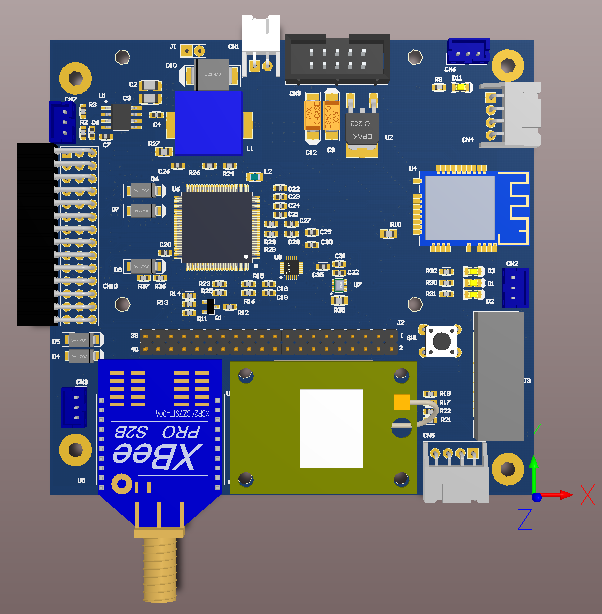
\includegraphics[width=\textwidth]{Img/BaseBoardV2_1.png}
    \caption{Plataforma base}
    \label{fig:baseboardv2_1}
\end{figure}

\subsubsection{Factor de forma}
En primer lugar, el tamaño de las plataformas suele ser un factor importante a la hora de querer conseguir una nueva. Por ello, los fabricantes generalmente siempre buscan tener el menor posible. Para este caso, como se hace hincapié en la versatilidad de la placa, se adopta el factor de forma PC104, en especial el PCIe104 OneBank, del cual se aprovechan las conectividades de SMBus y dos de USB. Debido a esto, el tamaño de la placa resulta ser de aproximadamente 10cmx10cm, haciendo que la placa no sea lo más pequeña posible, pero permitiendo entonces dicha versatilidad en base a un estándar ya definido.

\subsubsection{Alimentación}
Para poder alimentar la placa, el mismo permite hasta 18V de tensión de entrada, ya que cuenta con el regulador Buck sincrónico TPS54627\footnote{\url{http://www.ti.com/lit/ds/symlink/tps54627.pdf}}, el cual entrega una tensión de 5V y permite hasta 6A de corriente. De la salida del mismo se cuenta con un conector de alimentación para, por ejemplo, poder alimentar una Raspberry Pi sin necesidad de otra entrada de alimentación para la misma\footnote{Dichos microprocesadores suelen recomendar una alimentación de 3A promedio, el cual depende de los periféricos conectados a la misma, quedando en el peor de los casos 3A para el uso de la placa base en sí con todos sus perisféricos adicionales.}. Cabe destacar que, en caso que se tenga una Raspberry Pi montada en el conector pensado para la misma, en consecuencia no se podrá tener el una placa con factor de forma PC104 en la parte superior de la misma por temas de espaciado entre ellas.

\subsubsection{Unidad de procesamiento}
Si bien para el trabajo presente es necesario de un microprocesador para realizar tareas de alto rendimiento, tal como la recolección de imágenes de una cámara estéreo, en la presente se incluye como base un microcontrolador Cortex-M4, ya que el mismo está pensado para utilizarse en las tareas críticas del robot, como puede ser un control básico. Si bien para un robot terrestre esto puede no ser necesario, en el caso de querer realizar un drone, por ejemplo, la estabilidad del mismo al estar en vuelo es vital para evitar inconvenientes. En caso que se requiera mayor poder de cómputo, la placa cuenta cun una base para montar una Raspberry Pi compatible. Mas allá de que muchas de las plataformas vistas en la Sección \ref{sec:platforms} cuentan sólo con microprocesadores, se pretende en este caso aumentar la tolerancia a fallos al separar las tareas en dos unidades de procesamiento distintas, enfocando una de ellas a las tareas de control y funciones básicas, y la otra, por ejemplo, a realizar el SLAM.

\subsubsection{Conectividad}
Como se anticipó anteriormente, el mismo cuenta con el estándar de Hardware PCIe/104 OneBank, contando con comunicaciones de SMBus y USB por el mismo. Además de esto, el mismo dispone de conectores para
\begin{itemize}
    \item UART
    \item I2C
    \item GPIOs, además de salidas PWM con conectores propios pensadas para utilizar en distintos ESCs o controladores de motores
    \item Cuenta con pines específicos para montar una placa Raspberry Pi compatible, utilizando como medios de comunicaciones entre las mismas los protocolos UART e I2C.
\end{itemize}

\subsubsection{Sensores integrados}
Como existe una gran cantidad de sensores distintos dentro de las aplicaciones robóticas, en la placa base se montaron los más utilizados en las plataformas estudiadas en la Sección \ref{sec:platforms}.
\paragraph{Unidad de medición inercial (IMU)}
Siendo la IMU el sensor más utilizado dentro de la robótica aérea para el control del mismo, este sensor puede ser utilizado para un gran número de aplicaciones distintas, como por ejemplo para la corrección de la señal de GPS para calcular la posición del robot \textbf{(REF GPS IMU)}. Si bien existe una gran cantidad de IMUs distinta, tanto sea a nivel precio como en base a la cantidad de sensores que tengan (acelerómetro-giróscopo, acelerómetro-giróscopo-magnetómetro), dentro de la placa se dispone de una MPU9250\footnote{\url{https://invensense.tdk.com/wp-content/uploads/2015/02/PS-MPU-9250A-01-v1.1.pdf}}, la cual cuenta con nueve grados de libertad (9 \textit{degrees of freedom - DOF}), ya que posee un juego de acelerómetro, giróscopo y magnetómetro de tres ejes cada uno. Este integrado es una mejora del MPU6050, el cual se trata de un un giróscopo y un acelerómetro (6 DOF), resultando entonces en un \textit{multi-chip module} (MCM) de dos obleas, una correspondiente a un acelerómetro y un giróscopo, y la otra corresponde al magnetómetro AK8963. En concreto, las orientaciones de referencia de ambas obleas difieren, como puede verse en la Figura \ref{fig:mpu9250orientations}. Como se trata de un sensor de bajo costo, el mismo no suele tener todos sus sensores alineados correctamente.
\begin{figure}
    \centering
    \subfloat[Orientación de la oblea correspondiente al giróscopo  y el acelerómetro]{{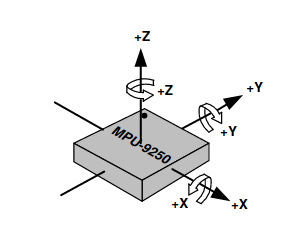
\includegraphics[width=0.45\textwidth]{Img/MPU9250GyroAccel.png}}}%
    \qquad
    \subfloat[Orientación de la oblea correspondiente al magnetómetro]{{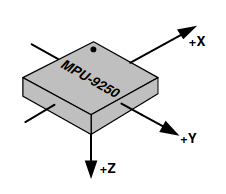
\includegraphics[width=0.45\textwidth]{Img/MPU9250Mag.png}}}%
    \caption{Orientaciones dentro del integrado MPU9250}
    \label{fig:mpu9250orientations}
\end{figure}

Generalmente, es recomendable que la IMU se encuentre en el centro de masa del robot. Sin embargo, debido a que la placa puede personalizarse con el agregado de módulos externos, se eligió el centro de coordenadas de la placa para la ubicación de la IMU.

\paragraph{Barómetro}
Si bien para el trabajo presentado puede no ser de utilidad, los barómetros son muy utilizados en los vehículos aéreos, ya que debido a las alturas elevadas que pueden alcanzar, el uso de un ultrasonido para medir la distancia al suelo sirve sólo para una corta distancia, mientras que los barómetros económicos son útiles a considerables alturas, siendo ambos métodos utilizados para tal fin. Al igual que el magnetómetro, la medición del barómetro respecta a una magnitud externa al robot, la presión atmosférica, y los datos del mismo suelen utilizarse en combinación con una IMU para conseguir una mejor estimación de la altitud\textbf{(Tanigawa, 2008)}, así como también para corregir la estimación de altitud del GPS\textbf{(Zaliva, 2014)}.

En concreto, para la placa se optó por el uso del barómetro BMP280\footnote{\url{https://cdn-shop.adafruit.com/datasheets/BST-BMP280-DS001-11.pdf}}, el cual es una mejora de su predecesor, el BMP180, aunque ambos tienen una precisión de aproximadamente un metro.

\paragraph{GPS}
Si bien el circuito integrado no se encuentra soldado en la placa base, en la misma se encuentra un soporte para poder colocar el módulo U-Blox GPS NEO6MV2, observada en la Figura \ref{fig:gpsneo6mv2}, el cual puede conseguirse fácilmente en el mercado local, aunque, como el resto de los sensores utilizados, presenta un error considerable en caso de que se quiera utilizarlo en soledad para calcular la posición global del robot, además de contar con una frecuencia de datos máxima de $1Hz$.
\begin{figure}
    \centering
    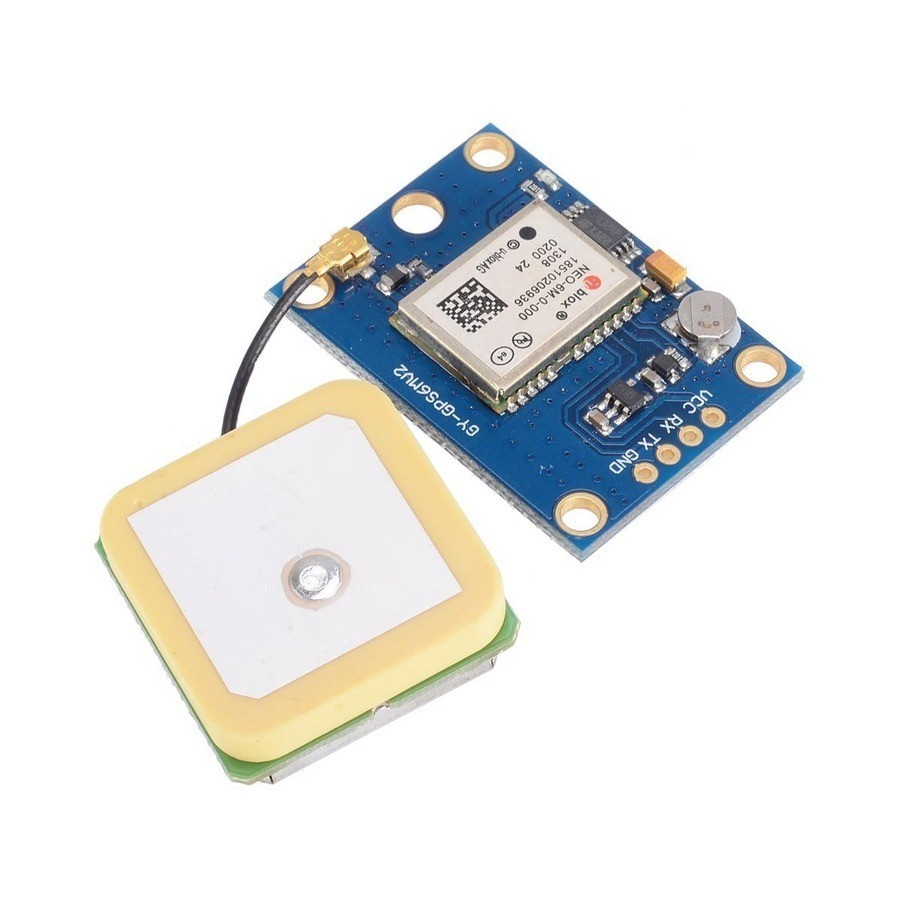
\includegraphics[scale=0.2]{Img/GPSNEO6MV2.jpg}
    \caption{Módulo U-Blox GPS NEO6MV2}
    \label{fig:gpsneo6mv2}
\end{figure}

\subsubsection{Sensores externos}
Si bien los sensores pueden agregarse mediante cualquiera de los pines de conectividad presentes en la placa, el mismo cuenta con la posibilidad de utilizar la interfaz DCMI, común en cámaras de baja resolución. Esto pude ser de utilidad en caso que se quiera tomar imágenes sólo con el uso del microcontrolador presente en la placa base.

Como gran parte de las aplicaciones robóticas cuentan con más de dos ultrasonidos, en la placa existen pines específicos para conectar hasta cinco de los mismos, ya que si bien la señal de Trigger para cada uno de los ultrasonidos es independiente, la señal de Echo es compartida, teniendo sólo que controlar un sólo pin, y en base a la señal de Trigger enviada puede conocerse cúal de ellos fue el que respondió. En caso que se requieran agregar más de estos sensores, puede hacerse utilizando los GPIOs disponibles.
\subsubsection{Sistemas de comunicaciones}
Para poder comunicar al robot, el mismo cuenta con
\begin{itemize}
    \item El módulo WiFi ATWINC1500\footnote{\url{http://ww1.microchip.com/downloads/en/DeviceDoc/ATWINC15x0-MR210xB-IEEE-802.11-b-g-n-SmartConnect-IoT-Module-Data-Sheet-DS70005304C.pdf}}, el cual es un módulo de bajo consumo bajo el estándar IEEE 802.11, conectado al microcontrolador mediante SPI.
    \item El módulo XBee-PRO S2C\footnote{\url{https://www.digi.com/resources/documentation/digidocs/pdfs/90002002.pdf}} mediante UART que, a diferencia del módulo WiFi, se trata de la versión Through-Hole, debido a la complicación que presentaba incluir su versión SMD y cumplir con los requisitos del estándar PC104.
    \item Al tener varios GPIOs disponibles, puede utilizarse un gran número de conectividades para radiocontrol (RC), tales como PPM y PWM. A su vez, se cuenta con la capacidad de incorporar un sistema Futaba S.Bus, ya que cuenta con un inversor de señal en una de sus entradas de UART. Sin embargo, para todos ellos es necesario agregar el receptor requerido.
\end{itemize}


\subsection{Robot desarrollado}
Antes de poder llegar al modelo final del robot, primero deben abordarse los aspectos considerados necesarios para la elaboración del mismo.

\subsubsection{Unidad de procesamiento}
Para que el robot pueda realizar tareas de SLAM, el mismo requiere de sensores exteroceptivos, en concreto de un LIDAR y una cámara estéreo, por lo que la unidad de procesamiento base (el Cortex-M4) no sería suficiente. Por ello, se adiciona al soporte específico del mismo una Raspberry Pi 4, buscando no sólo poder recolectar la información de estos sensores, sino también extender la capacidad de cómputo.

\subsubsection{Sensores útiles integrados en la plataforma base}
Como se pretende utilizar la placa base presentada anteriormente, ya que se busca realizar un robot terrestre, de la misma para el desarrollo de SLAM es de interés especialmente la IMU integrada en el mismo, dejando de lado el barómetro por no despegarse del piso. Si bien el GPS puede ser de gran utilidad para calcular la posición georeferenciada, se pretende poder realizar un \textit{SLAM indoor}, esto es, un SLAM dentro de un espacio cerrado, donde la señal de GPS se encuentra denegada.

\subsubsection{Módulos y sensores externos}
Como se mencionó anteriormente, en el robot se pretende utilizar un LIDAR y una cámara estéreo como sensores extereoceptivos. Como los mismos suelen ser costosos, se utilizaron provistos por la facultad, los cuales son
\begin{itemize}
    \item Scanse Sweep Laser Scanner\footnote{\url{https://s3.amazonaws.com/scanse/Sweep_user_manual.pdf}} (Figura \ref{fig:externalmodulesandsensors}.a): Se trata de un sensor LIDAR montado sobre una pieza giratoria, permitiendo entonces el sensado en 360 grados. Cuenta con una recolección de 1000 muestras por segundo, con un rango máximo de hasta 40 metros segun especificación. La frecuencia de escaneo máxima respecta a 10Hz.
    \item Minoru 3D Webcam\footnote{\url{https://www.robotshop.com/media/files/pdf/user-guide-3d-webcam.pdf}} (Figura \ref{fig:externalmodulesandsensors}.b): Se trata de una cámara estéreo, la cual se comunica mediante USB 2.0, presentando entonces un compromiso de resolución-marcos por segundo debido a la transferencia máxima del protocolo. Las cámaras no se encuentran sincronizadas, teniendo un desvío máximo de 16.5ms.
\end{itemize}
\begin{figure}
    \centering
    \subfloat[Scanse Sweep Laser Scanner]{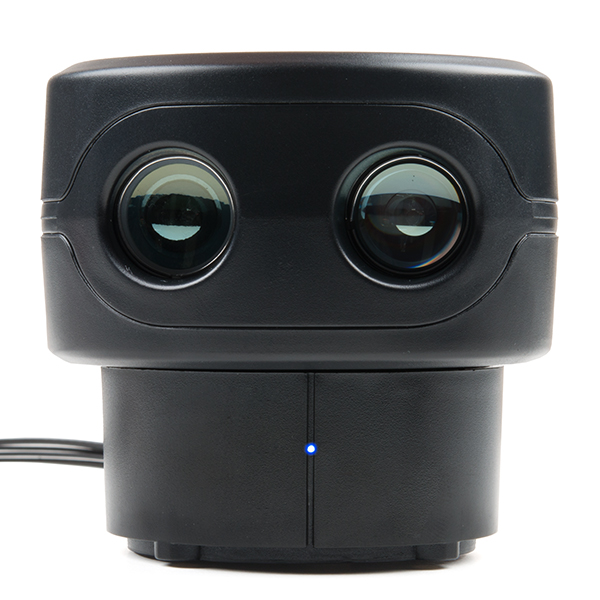
\includegraphics[width=0.2\textwidth]{Img/scanse-sweep.jpg}}
    \qquad
    \subfloat[Minoru Webcam]{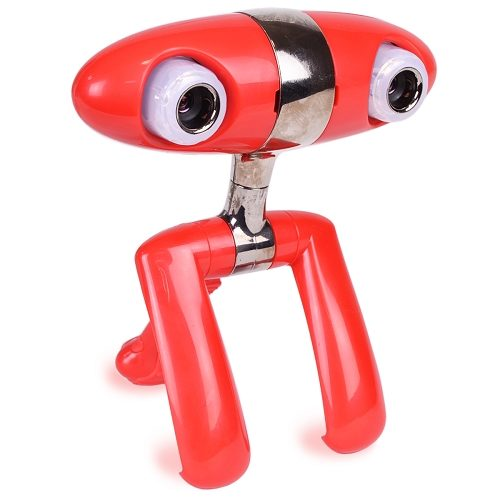
\includegraphics[width=0.2\textwidth]{Img/Minoru.jpeg}}
    \qquad
    \subfloat[Móudlo LM298]{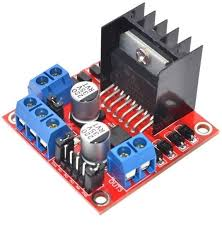
\includegraphics[width=0.2\textwidth]{Img/LM298.jpeg}}
    \qquad
    \subfloat[Móudlo LM2596]{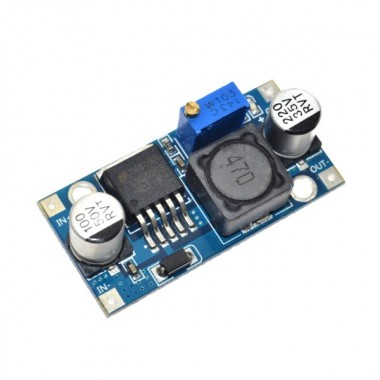
\includegraphics[width=0.22\textwidth]{Img/LM2596.jpeg}}
    \caption{Módulos y sensores externos}
    \label{fig:externalmodulesandsensors}
\end{figure}

Como es necesario poder controlar los motores, se incluyó un puente H para proveer a los mismos, utilizando el módulo comercial LM298, correspondiente a la Figura \ref{fig:externalmodulesandsensors}.c. Como la placa base proporciona una tensión regulada de 5V, para el puente H esto no es de gran utilidad, ya que el mismo requiere de 6 a 12V de alimentación. Para poder solucionar esto, se agregó también un módulo regulador del LM2596 ajustable, como el de la Figura \ref{fig:externalmodulesandsensors}.d.

\begin{figure}
    \centering
    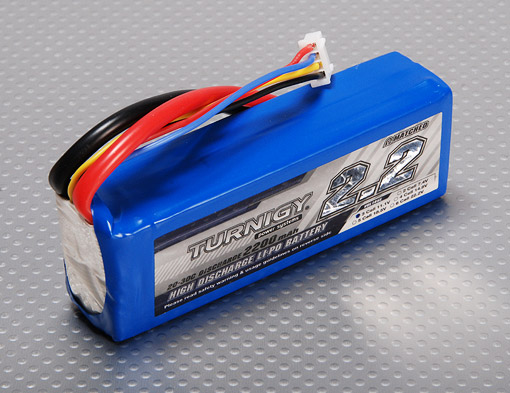
\includegraphics[width=0.5\textwidth]{Img/LiPo3S.jpg}
    \caption{Batería LiPo comercial utilizada en diferentes robots}
    \label{fig:lipobattery}
\end{figure}
\subsubsection{Estructura}
Siendo que tanto los sensores como la placa son relativamente voluminosos, es necesario que la estructura del robot permita ubicarlos a todos ellos sin estorbarse entre sí. Además de esto, al disponer de una batería LiPo de 3 celdas (Figura \ref{fig:lipobattery}), la misma debe tener un espacio dedicado no sólo para poder ubicarla, sino también que ofrezca algún tipo de resguardo, para evitar daños debido a efectos indeseados y corriendo el riesgo de que la misma pueda deteriorarse. Por estos motivo, se optó por el uso del chasis Auto Robot Smart Car 4WD, el cual cuenta con cuatro ruedas y motores, como se observa en la Figura \ref{fig:developedrobot}.a.
\begin{figure}
    \centering
    \subfloat[Chasis elegido para el robot terrestre]{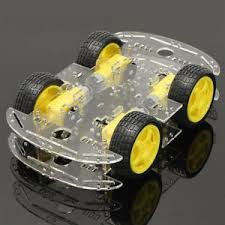
\includegraphics[width=0.45\textwidth]{Img/AutoRobotSmartCar4WD.jpeg}}
    \qquad
    \subfloat[Robot con piezas 3D montadas]{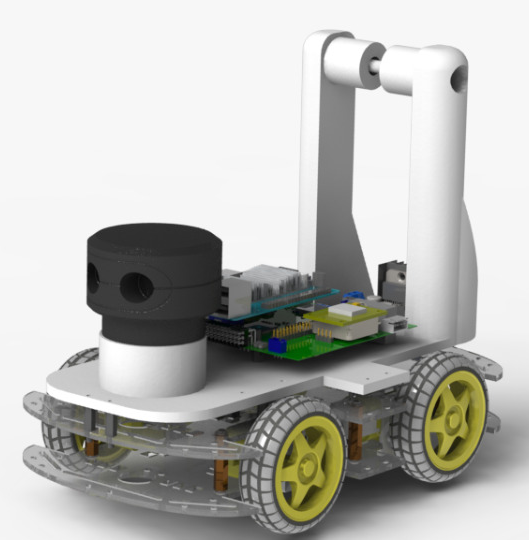
\includegraphics[width=0.45\textwidth]{Img/3DRobot.png}}
    \caption{Robot desarrollado}
    \label{fig:developedrobot}
\end{figure}

Para poder ubicar todos los componentes en la placa, es necesario que la cámara estéreo se encuentre distanciada del suelo, caso contrario dificultaría la triangulación debido al offset de cada una de las cámaras. A su vez, es preferible que el LIDAR tenga la menor cantidad de obstáculos posibles en el camino del láser, consiguiendo así una mayor cantidad de puntos útiles por barrido. A partir de esto, con el uso de una impresora 3D se desarrollaron piezas para cumplir con los requisitos, centrando la placa base en el centro del robot, tal como puede observarse en la Figura \ref{fig:developedrobot}.b. 





\subsection{Calibración de la unidad inercial de medición}
Para la calibración de la unidad inercial presente en el robot, esto es, el MPU9250, se realizó una base de madera fija, con el fin de poder moverlo con mayor facilidad. A su vez, como puede observarse en la Figura \ref{fig:baseboardimucalibrationwithframe}, se montó sobre la placa base una Raspberry Pi mediante el uso de \texttt{rosserial}, y se conectó esta Raspberry con la red WiFi para poder recolectar datos mediante ROS (guardándolos mediante el uso de \texttt{rosbag}), evitando el uso de cables externos, exceptuando al de alimentación.
\begin{figure}
    \centering
    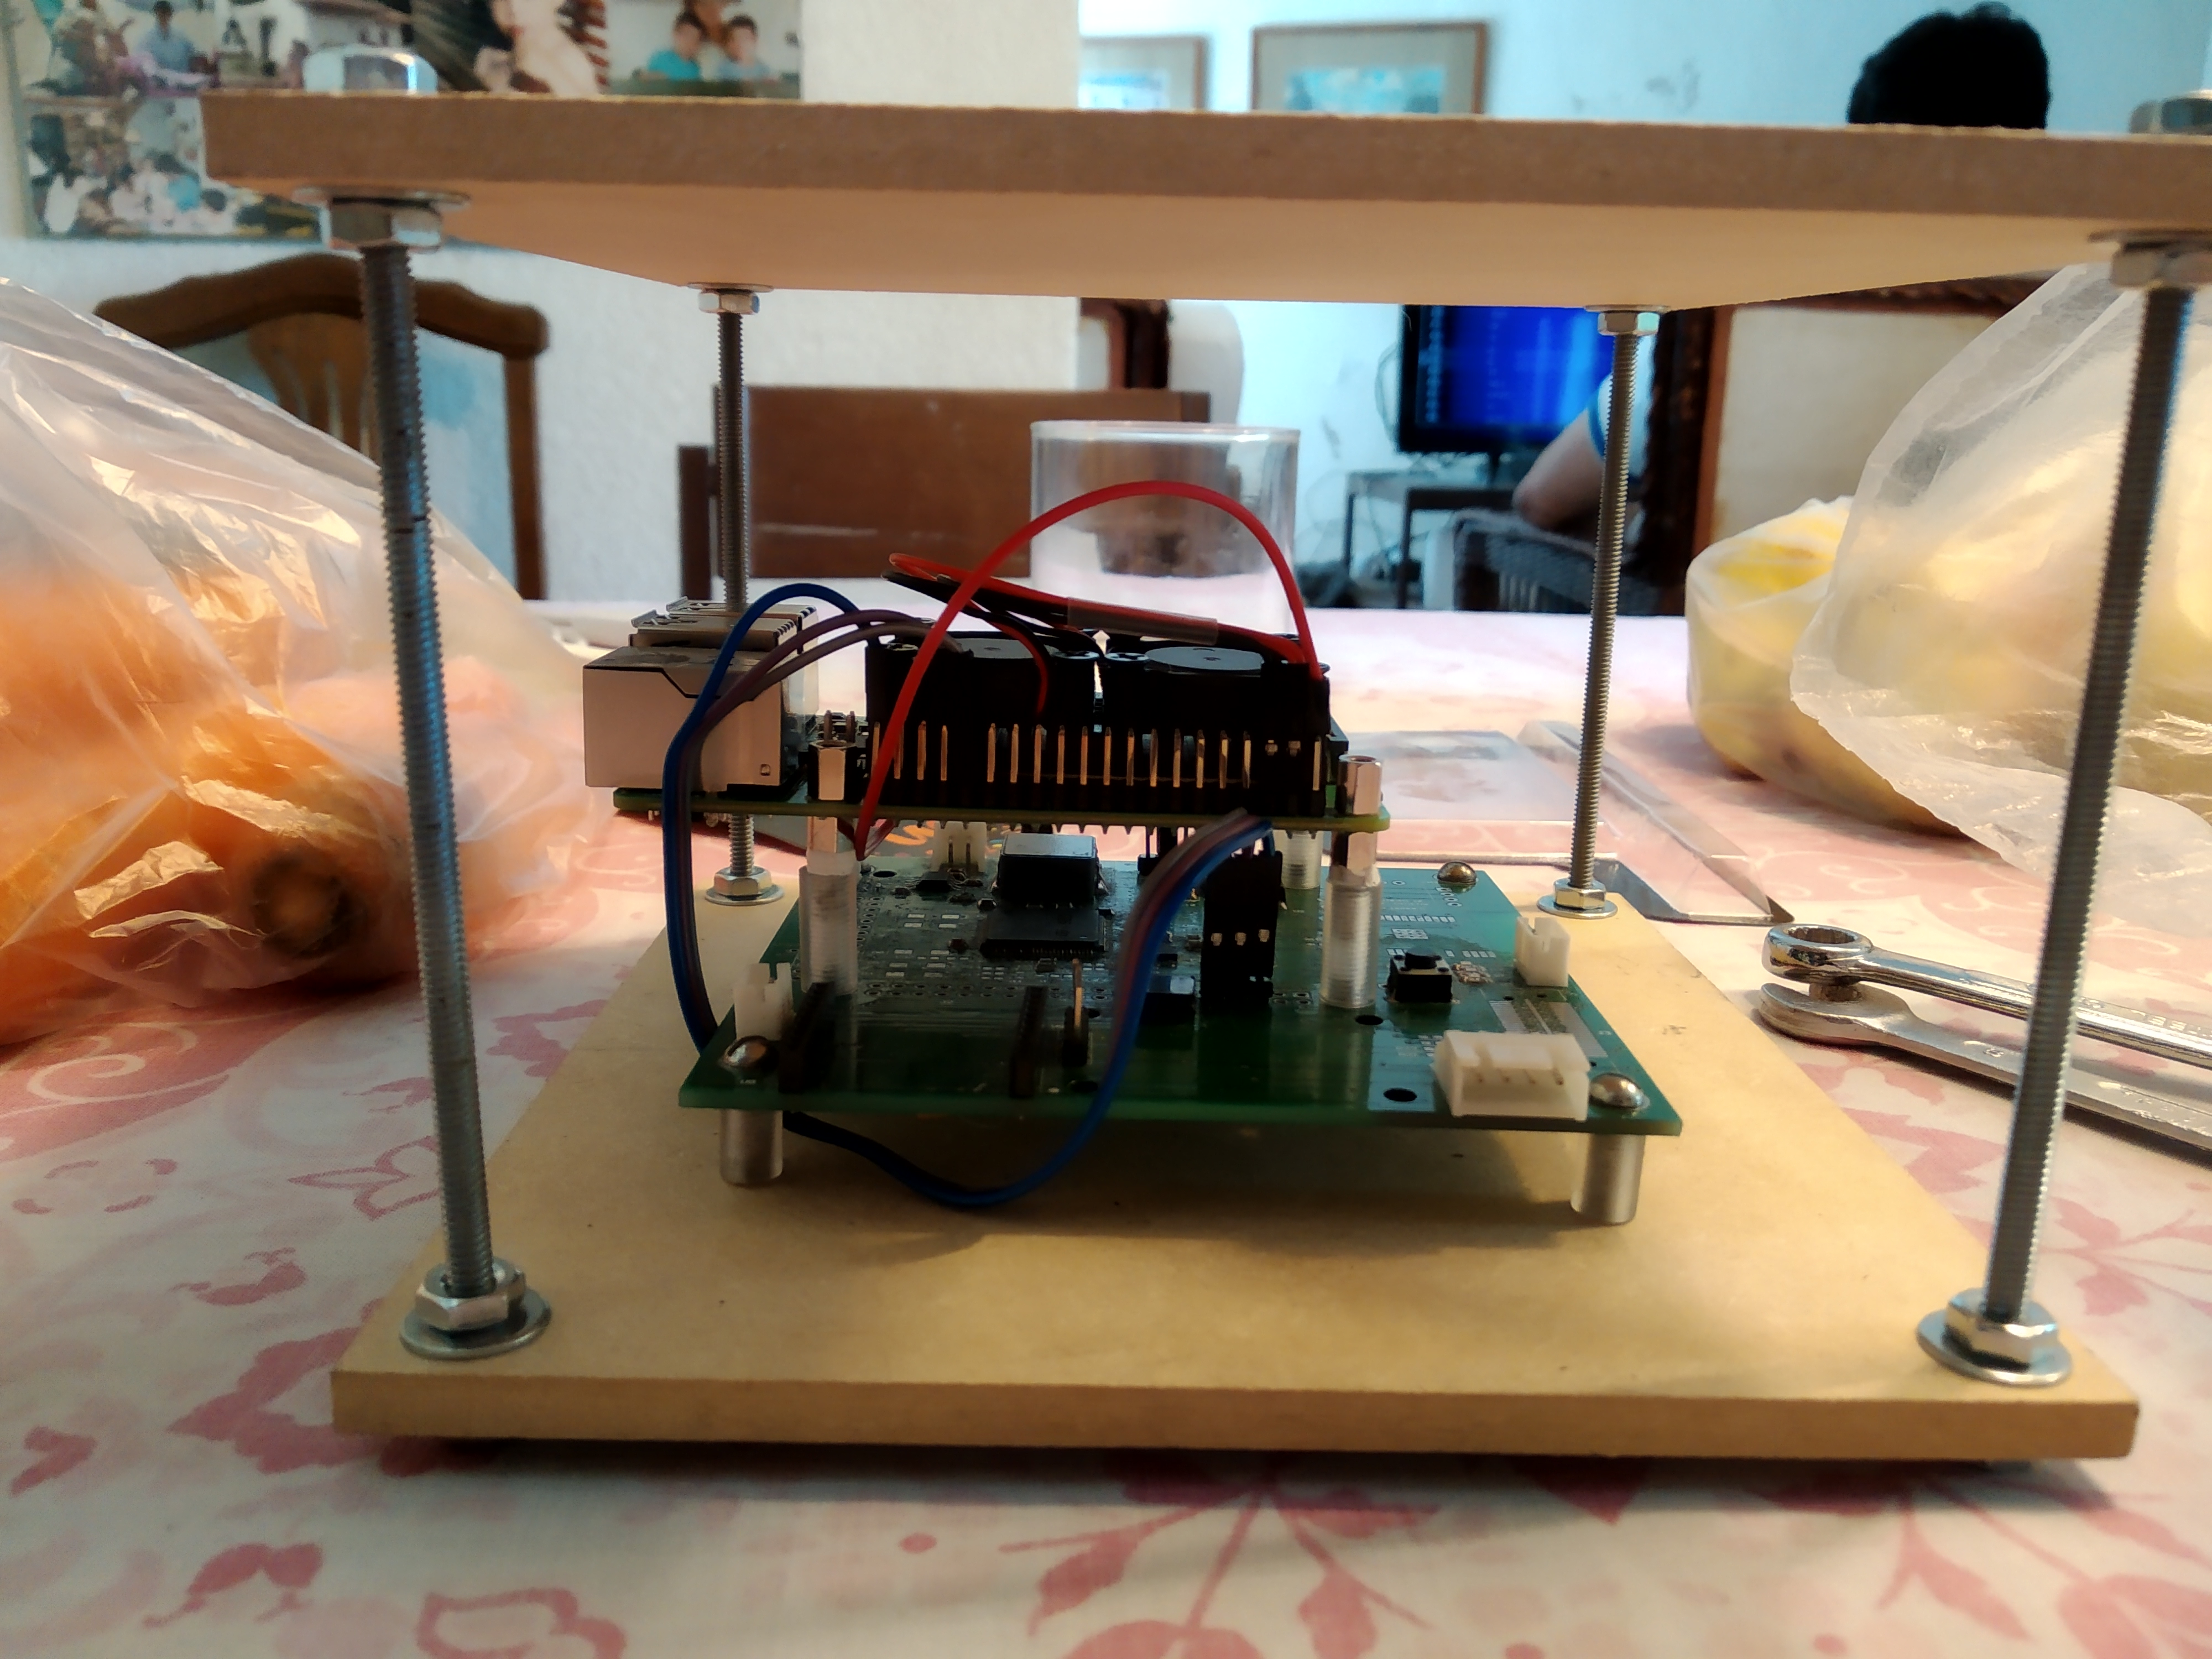
\includegraphics[width=\textwidth]{Img/BaseBoardIMUCalibrationWithFrame.jpg}
    \caption{Placa base con una Raspberry Pi sobre un marco fijo}
    \label{fig:baseboardimucalibrationwithframe}
\end{figure}


\subsubsection{Calibración del acelerómetro y giróscopo}
Tal como se desarrolló en la Sección \ref{sec:sensors}, la calibración del giróscopo se encuentra ligada a la calibración del acelerómetro, por lo que una mala calibración del acelerómetro hará llevará a una calibración inexacta del giróscopo. Además, como se pretende utilizar el mismo dataset para calibrar a ambos sensores, es necesario poder estimar todas las variables previas necesarias para tal fin.

\paragraph{Varianza de Allan para el cálculo de $T_{init}$}
Para poder conocer el tamaño adecuado que permita obtener el \textit{bias} del giróscopo en el instante inicial, se utiliza la \textit{varianza de Allan}[20][8] $\sigma_{Allan}$, la cual mide la varianza de la diferencia entre promedios de intervalos consecutivos, siendo entonces
\begin{align}
    \sigma_{Allan} &= \frac{1}{2} E[(x(\tilde{t},k) - x(\tilde{t},k-1))^2] \\
    &= \frac{1}{2K}\sum_{k=1}^K(x(\tilde{t},k) - x(\tilde{t},k-1))^2
\end{align}
donde $x(\tilde{t},k)$ es el \textit{k-ésimo} intervalo promedio que abarca $\tilde{t}$ segundos, y K es el número de intervalos en que se segmenta el tiempo total considerado. Se computa la varianza de Allan para los tres ejes del giróscopo, y en el intervalo de tiempo en el que los tres convergen a un valor pequeño representa una buena elección para elegir el período de inicialización, $T_{init}$.

Para el banco de ensayos presentado anteriormente, se tomaron mediciones de la unidad sin movimiento alguno pro un largo período de tiempo, obteniendo con la varianza de Allan las curvas de la Figura \ref{fig:imugyrovariance}. En la misma, puede observarse que un valor en el cual convergen las tres mediciones es alrededor de
\begin{equation}
    T_{init} = 8 s
\end{equation}
siendo este entonces el elegido.
\begin{figure}
    \centering
    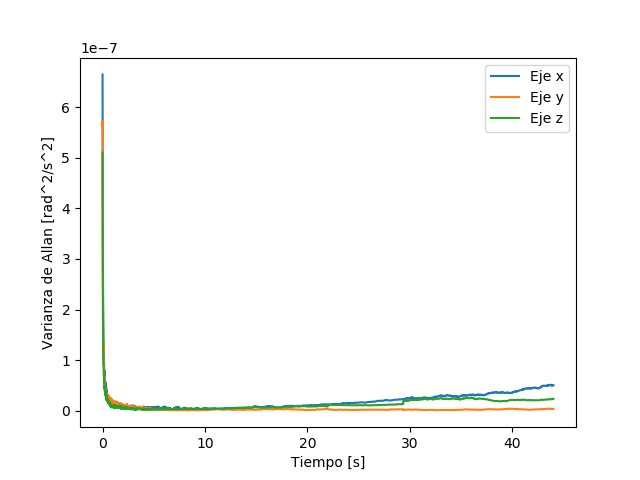
\includegraphics[width=\textwidth]{Img/IMUGyroVariance.png}
    \caption{Varianza de Allan para determinar el $T_{init}$ necesario para calcular el bias del giróscopo}
    \label{fig:imugyrovariance}
\end{figure}

\paragraph{Detector estático}
Como lo que se busca es promediar los datos del acelerómetro cuando el mismo permanece estático, es necesario poder entonces determinar en que momento el banco de pruebas se encuentra inmóvil. Tal como en \textbf{(Tedaldi, 2014)}, se propone el uso de un detector estático basado en la varianza de la aceleración, promediando cada un cierto tiempo $t_p$
\begin{equation}
    \xi(t) = \sqrt{(var_{t_p}\ a_x(t))^2 + (var_{t_p}\ a_y(t))^2 + (var_{t_p}\ a_z(t))^2}
\end{equation}
y luego compararlo con un cierto umbral para verificar de que se trate de un intervalo estático o no. Para ello, aprovechando el $T_{init}$ necesario en la calibración del giróscopo, se calcula primero un $\xi_{init}$ basado en el cálculo de la Expresión para el intervalo de tiempo mencionado, y luego, para cada instante de tiempo, si
\begin{equation}
     k\xi^2(t) < \xi^2_{init}
\end{equation}
el intervalo corresponderá a un estático, caso contrario se tratará de uno en movimiento. El parámetro $k$ se trata de un ajuste empírico para lograr mejores resultados.

Si bien el tiempo estático en que puede estar el banco para la calibración del acelerómetro puede ser extenso\footnote{Mientras más muestras se tengan, mejor será el promediado, aunque produce que se requiera más tiempo de procesamiento}, para el giróscopo es importante de que no alcance un tiempo mayor al expresado por la varianza de Allan, ya que indicaría que el mismo se encontraría en estado estacionario. Por ello, como se busca que el $T_init$ pueda ser expresado en base a los $t_p$ se adopta a este último con
\begin{equation}
    t_p = 1 s
\end{equation}

\paragraph{Calibración del acelerómetro}
En base a todos los parámetros calculados anteriormente, se tomaron las mediciones de la unidad inercial de medición, dejándola primero estática por aproximadamente $T_{init}$, y luego ubicándola en diferentes rotaciones con intervalos estáticos entre las mismas de menos de $T_{init}$. Como se tienen nueve parámetros para poder calibrar tanto el acelerómetro como el giróscopo (detallados en la Expresiones (\ref{eq:accelcalibrationparams}) y (\ref{eq:gyrocalibrationparams})\footnote{Mínimamente se necesitan la misma cantidad de mediciones que de incógnitas, aunque mientras más mediciones haya, mejor será la estimación}), se realizan un gran número de posiciones, obteniendo entonces las aceleraciones observadas en la Figura \ref{fig:imugyroaccelcal}. Junto a dichos datos, se representa el detector de estáticos, ajustado con un
\begin{equation}
    k = 2.0
\end{equation}
\begin{figure}
    \centering
    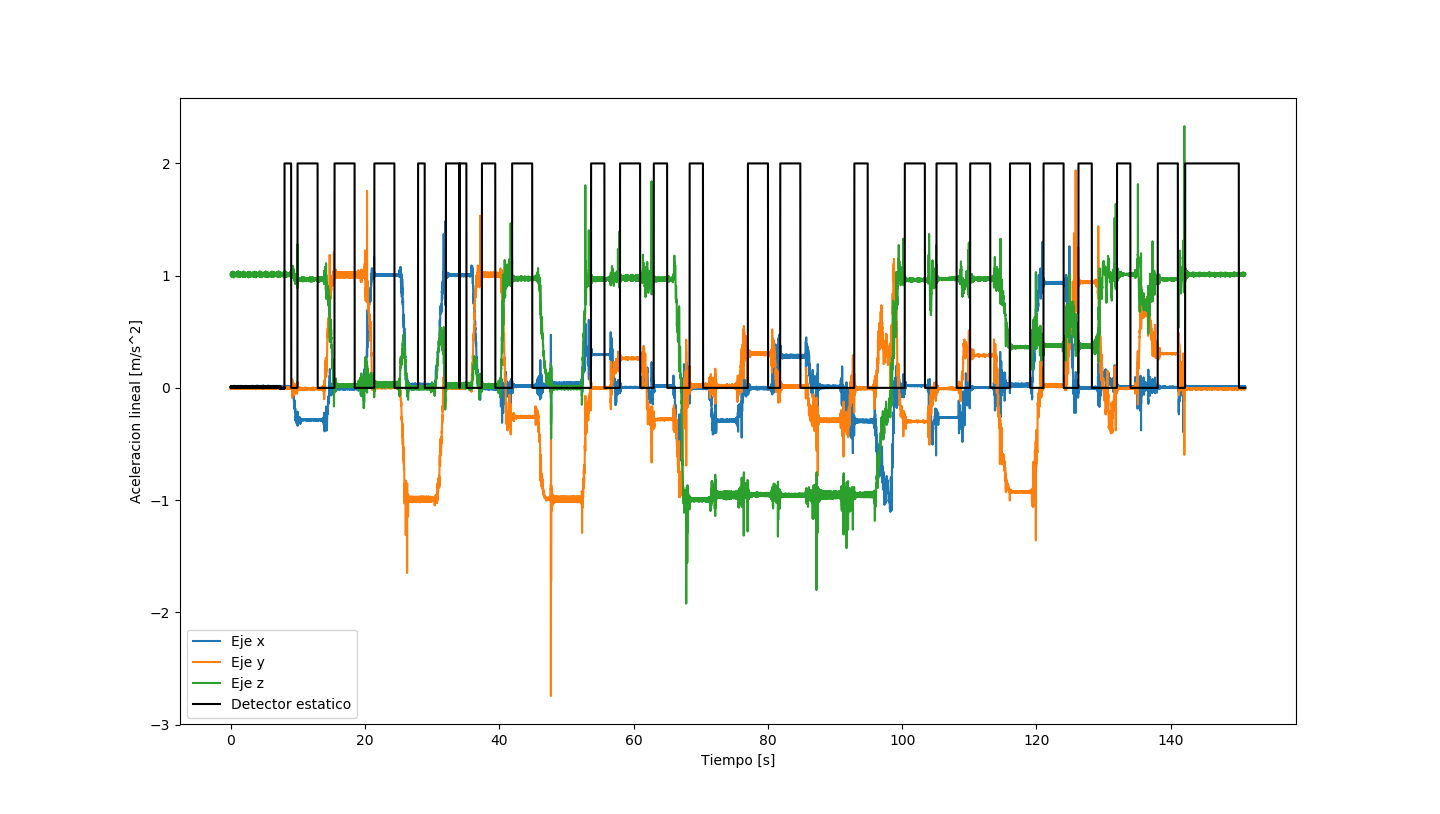
\includegraphics[width=\textwidth]{Img/IMUGyroAccelCal.png}
    \caption{Datos obtenidos del acelerómetro para utilizar en la calibración, incluyendo el detector de estáticos}
    \label{fig:imugyroaccelcal}
\end{figure}

En base a los intervalos estáticos, se procede al promediado de los intervalos, para luego utilizarlos en la función de coste de la Expresión (\ref{eq:generalaccelcostfunction}). Como para este caso particular los datos obtenidos del acelerómetro se encuentran normalizados, dicha Expresión puede simplificarse a la forma
\begin{equation}
    \mathscr{S}(\bm{\epsilon}_{a}) = \sum_{k=1}^M(1-||h(\bm{a}^s_k,\bm{\epsilon}_{a})||^2)^2
    \label{eq:mpu9250accelcostfunction}
\end{equation}
minimizándola mediante el algoritmo de Levenbeg-Marquandt, en base a los intervalos estáticos promediados. De la misma, se obtuvieron los siguientes parámetros
\begin{align}
        \bm{C}_a &=
    \begin{bmatrix}
        1 & -0.0369903 & -0.00491802 \\
        0 & 1 & -0.00370494 \\
        0 & 0 & 1
    \end{bmatrix}
    \\
        \bm{K}_a &=
    \begin{bmatrix}
        1.00014 & 0 & 0 \\
        0 & 0.999156 & 0 \\
        0 & 0 & 0.995609
    \end{bmatrix}
    \\
    \bm{b}_a &=
    \begin{bmatrix}
        -0.00401076 \\
        -0.00737427 \\
        -0.00671314
    \end{bmatrix}
\end{align}

\paragraph{Integración de la velocidad angular}
Como se desarrolló en la Sección \ref{sec:sensors}, la integración de la velocidad angular utilizando cuaterniones no es una tarea sencilla.
Esta función, en concreto, requiere de una integración de la velocidad angular en un tiempo discreto. Si bien existen diferentes métodos de integración numérica, es necesario que el mismo sea robusto y estable para mejorar la exactitud de la calibración. Por eso, el \textit{Runge-Kutta} $4^{th}$ \textit{order normalized method} (RK4n)\textbf{(Vojtesek, 2014)} es el elegido, aunque existen otros métodos que pueden utilizarse para este fin \textbf{(Andrle, 2013)}.

Si la ecuación diferencial que describe a la cinemática del cuaternión se define como
\begin{equation}
    \bm{f}(\bm{q},t) = \dot{\bm{q}} = \frac{1}{2}\bm{\Omega}(\bm{\omega}(t))\bm{q}
\end{equation}
donde $\bm{\Omega}(\bm{\omega}(t))$ es el operador que convierte la velocidad angular tridimensional considerada en la representación de la matriz simétrica oblicua real, esto es,
\begin{equation}
    \bm{\Omega}(\bm{w}) = 
    \begin{bmatrix}
        0 & -w_x & -w_y & -w_z \\
        w_x & 0 & w_z & -w_y \\
        w_y & -w_z & 0 & w_x \\
        w_z & w_y & -w_x & 0
    \end{bmatrix}
\end{equation}
El algoritmo de integración RK4n es
\begin{align}
    \bm{q}_{k} &= \bm{q}_{k-1} + \Delta t\frac{1}{6}(\bm{k}_1 +\bm{k}_2 + \bm{k}_3 + \bm{k}_4) \\
    \bm{k}_i &= \bm{f}(\bm{q}^{(i)},t_{k-1}+c_i\Delta t) \\
    \bm{q}^{(i)} &= \bm{q}_{k-1} &&\text{para} &&&i=1 \\
    \bm{q}^{(i)} &= \bm{q}_{k-1} + \Delta t\sum_{j=1}^{i-1}a_{ij}\bm{k}_j &&\text{para} &&&i>1
\end{align}
donde todos los coeficientes necesarios, $c_i$ y $a_{ij}$ son
\begin{align*}
    c_1 &= 0,\ c_2 = \frac{1}{2},\ c_3 = \frac{1}{2},\ c_4 = 1 \\
    &a_{21} = \frac{1}{2},\ a_{31} = 0,\ a_{41} = 0, \\
    &a_{32} = \frac{1}{2},\ a_{42} = 0,\ a_{43} = 1
\end{align*}

Finalmente, en cada paso, es necesario normalizar el cuaternión \textit{(k+1)-ésimo}, ya que puede exceder el valor unitario
\begin{equation}
    \bm{q}_{k+1} \rightarrow \frac{\bm{q}_{k+1}}{||\bm{q}_{k+1}||}
\end{equation}

\paragraph{Calibración del giróscopo}
\textbf{REVISAR LOS k y k+1!!!!!!!!}
Una vez calibrado el acelerómetro, se procede a la calibración del giróscopo utilizando el mismo dataset. Para ello, en primer lugar se obtiene el bias de giróscopo mediante el promedio de cada eje en el instante inicial $T_{init}$, obteniendo entonces
\begin{equation}
    \bm{b}_g =
    \begin{bmatrix}
         -0.00145159 \\
         0.00136245 \\
         0.0196623
    \end{bmatrix}
\end{equation}

A partir de estos valores, se plantea la resolución de la ecuación diferencial ordinaria mediante el algoritmo RK4n, y luego al cuaternión resultante se lo transforma en una matriz de rotación $\bm{\Lambda}(\bm{q}_{k+1})$ para ser aplicada al versor gravedad
\begin{equation}
    \bm{u}_{a,k-1} = \bm{g} =
    \begin{bmatrix}
        0 \\
        0 \\
        1
    \end{bmatrix}
\end{equation}
obteniendo entonces
\begin{equation}
    \bm{u}_{g,k} = \bm{\Lambda}(\bm{q}_{k+1})\bm{g}
\end{equation}

Finalmente, se reemplaza dicha magnitud dentro de la función de coste
\begin{equation}
    \mathscr{S}(\bm{\epsilon}_{g}) = \sum_{k=2}^M ||\bm{u}_{a,k} - \bm{u}_{g,k}||^2
\end{equation}
la cual se minimiza utilizando el algoritmo de Levenberg-Marquandt. Del mismo, se obtienen las matrices
\begin{align}
        \bm{C}_g &=
    \begin{bmatrix}
        1 & 0.0568771 & 0.0558162 \\
        0.253165 & 1 & -0.0749733 \\
        0.0284105 & -0.103141 & 1
    \end{bmatrix}
    \\
        \bm{K}_g &=
    \begin{bmatrix}
        1.19264 & 0 & 0 \\
        0 & 0.97173 & 0 \\
        0 & 0 & 1.0037
    \end{bmatrix}
\end{align}

\subsubsection{Calibración del magnetómetro}
asdasdsa

\subsection{Calibración de la cámara estéreo}
Siguiendo la metodología explicada en la Sección \ref{sec:sensors}, para la calibración de la cámara Minoru se utilizó un chessboard de 8x6, con cuadrículas de 10,8cm de lado, tal como la matriz presentada en el tutorial de calibración estéreo del paquete \texttt{camera\_calibration}\footnote{\url{http://wiki.ros.org/camera_calibration/Tutorials/StereoCalibration}}. Siendo que tanto en ROS como en OpenCV los extremos se buscan horizontalmente, es recomendable presentar el chessboard con la mayor cantidad de bordes de manera horizontal, tal como se observa en las calibraciones instantáneas de la Figura \ref{fig:minorurightleft}.

\begin{figure}[!ht]
    \centering
    \subfloat{{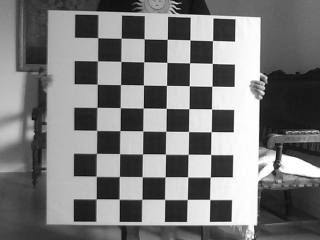
\includegraphics[width=0.45\textwidth]{Img/MinoruLeft.png}}}%
    \qquad
    \subfloat{{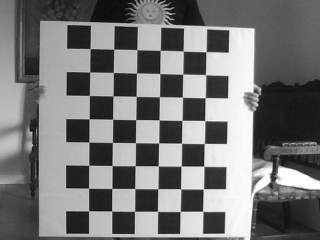
\includegraphics[width=0.45\textwidth]{Img/MinoruRight.png}}}%
    \caption{Imágenes izquierda y derecha de la calibración de la cámara Minoru}
    \label{fig:minorurightleft}
\end{figure}

Por razones de ancho de banda de USB 2.0, se configuraron las cámaras para trabajar en la resolución 320x240 a 30fps, consiguiendo entonces una imagen fluída, pero con una resolución limitada. A su vez, como la cámara utilizada no se encuentra sincronizada, es necesario realizar una aproximación entre ambas cámaras para tener mejores resultados en la calibración. Luego de un set de mediciones, se obtuvieron los datos de calibración de cada cámara, todos expuestos en dos archivos YAML, uno para la cámara derecha (Código \ref{lst:rightcamerayaml}) y otro para la cámara izquierda (Código \ref{lst:leftcamerayaml}).
\begin{lstlisting}[caption=YAML de la calibración de la cámara derecha mediante ROS, label=lst:rightcamerayaml]
image_width: 320
image_height: 240
camera_name: right_camera
camera_matrix:
  rows: 3
  cols: 3
  data: [ 435.736  ,    0.     ,  163.48678,
            0.     ,  436.74973,  117.12178,
            0.     ,    0.     ,    1.     ]
camera_model: plumb_bob
distortion_coefficients:
  rows: 1
  cols: 5
  data: [-0.139272, 0.228863, 0.000443, 0.002089, 0.000000]
rectification_matrix:
  rows: 3
  cols: 3
  data: [ 0.99997044, -0.00746816,  0.00182902,
          0.00746328,  0.99996861,  0.00266238,
         -0.00184884, -0.00264865,  0.99999478]
projection_matrix:
  rows: 3
  cols: 4
  data: [ 453.19158,    0.     ,  159.7411 ,  -27.55073,
            0.     ,  453.19158,  110.3157 ,    0.     ,
            0.     ,    0.     ,    1.     ,    0.     ]
\end{lstlisting}
\begin{lstlisting}[caption=YAML de la calibración de la cámara izquierda mediante ROS, label=lst:leftcamerayaml]
image_width: 320
image_height: 240
camera_name: left_camera
camera_matrix:
  rows: 3
  cols: 3
  data: [ 431.44958,    0.     ,  151.48809,
            0.     ,  432.60045,  103.73964,
            0.     ,    0.     ,    1.     ]
camera_model: plumb_bob
distortion_coefficients:
  rows: 1
  cols: 5
  data: [-0.088844, -0.120207, 0.001345, -0.002007, 0.000000]
rectification_matrix:
  rows: 3
  cols: 3
  data: [ 0.99989833, -0.0080206 , -0.01178974,
          0.00798926,  0.99996443, -0.0027027 ,
          0.011811  ,  0.00260823,  0.99992685]
projection_matrix:
  rows: 3
  cols: 4
  data: [ 453.19158,    0.     ,  159.7411 ,    0.     ,
            0.     ,  453.19158,  110.3157 ,    0.     ,
            0.     ,    0.     ,    1.     ,    0.     ]
\end{lstlisting}

\fi

\ifimagenes
\subsection{Experimentación con cámara estéreo}
Con el fin de utilizar datos reales, en principio se optó por usar la cámara estéreo Minoru 3D Webcam, la cual puede observarse en la Figura \ref{fig:minoru3dwebcam}. La misma cuenta con una interfaz USB 2.0 y una resolución de hasta 640x480, pudiendo además proporcionar hasta 30fps.
\begin{figure}
    \centering
    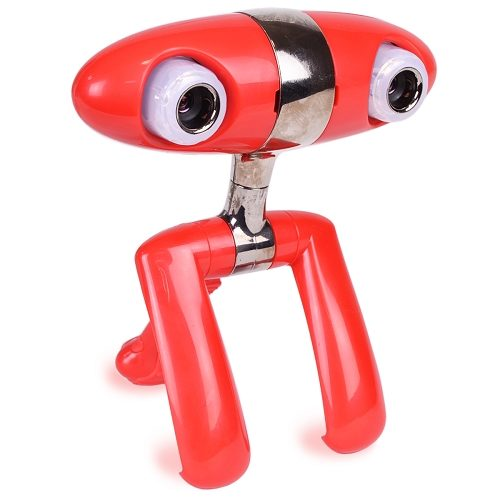
\includegraphics[width=0.2\textwidth]{Img/Minoru.jpeg}
    \caption{Cámara estéreo Minoru 3D Webcam}
    \label{fig:minoru3dwebcam}
\end{figure}

A pesar de estas especificaciones mencionadas anteriormente, no podría obtenerse una resolución de 640x480 a 30fps, debido a la limitación propia del USB 2.0. Por eso, se optó por trabajar con una resolución de 320x240 para poder mantener los fps.

\subsubsection{Calibración de la cámara}
Como la Minoru presenta la posibilidad de cambiar el enfoque de cada una de las cámaras monoculares, es necesario realizar una calibración de la misma cada vez que se realice un ajuste en dichos focos. Como en primera instancia se desconocía la calibración actual de dicha cámara, se optó por elegir un enfoque dado para luego calibrarla mediante el paquete de ROS \texttt{camera\_calibration}, presentado en la Sección \ref{sec:marcoteorico}. Para esto, se utilizó un chessboard de 8x6 con cuadrículas de 10,8cm de lado. Siendo que tanto en ROS como en OpenCV los extremos se buscan horizontalmente, es recomendable presentar el chessboard con la mayor cantidad de bordes de manera horizontal.

Luego de mover a la cámara en distintas orientaciones y consiguiendo por ende una buena cantidad de correlaciones entre las imágenes observadas en distintos patrones, se procede a la calibración de los datos obtenidos. Además de proveer con los archivos de calibración correspondientes, el paquete de ROS otorga las imágenes que fue tomando en cada caso (tanto izquierda como derecha) para cada una de las correspondencias que encontró en las imágenes. Por ejemplo, en la Figura \ref{fig:minorurightleft} puede observarse las vistas izquierda y derecha de cuando el algoritmo encontró una correspondencia entre ambas imágenes.

\begin{figure}[!ht]
    \centering
    \subfloat{{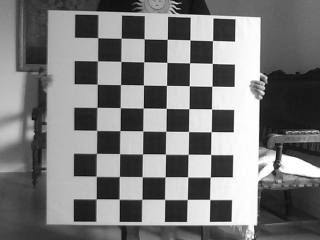
\includegraphics[width=0.45\textwidth]{Img/MinoruLeft.png}}}%
    \qquad
    \subfloat{{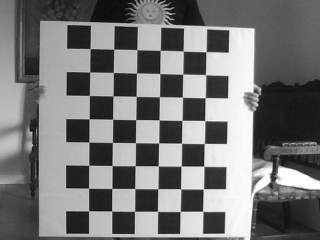
\includegraphics[width=0.45\textwidth]{Img/MinoruRight.png}}}%
    \caption{Imágenes izquierda y derecha de la calibración de la cámara Minoru}
    \label{fig:minorurightleft}
\end{figure}

\subsubsection{Nube de puntos obtenida}
Luego de la calibración, con el paquete de ROS \texttt{stereo\_image\_proc} se puede obtener el mapa de profundidades de la cámara. Además, como se mencionaba anteriormente, dicho paquete cuenta con una opción gráfica para poder configurar los parámetros de las correspondencias estéreo, facilitando la configuración del mismo. Finalmente, con dichos ajustes se obtiene la nube de puntos observada en la Figura \ref{fig:minorupointcloud}, donde en se encuentran las imágenes en crudo de las cámaras izquierda y derecha, la nube de disparidad calculada, y la nube de puntos final obtenida.

\begin{figure}[!ht]
    \centering
    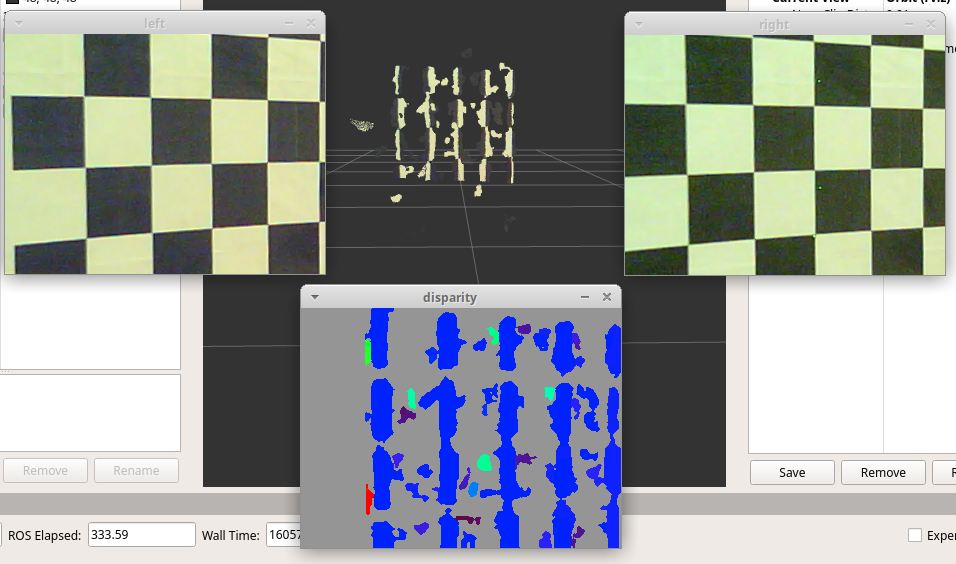
\includegraphics[width=\linewidth]{Img/MinoruPointCloud.png}
    \caption{Imágenes izquierda y derecha, disparidades y nube de puntos conseguida a partir de la cámara Minoru}
    \label{fig:minorupointcloud}
\end{figure}

Si bien la nube de puntos adquirida por el sensor presenta discontinuidades, con el procesamiento adecuado puede mitigarse este problema. Sin embargo, como las cámaras no están sincronizadas por hardware entre sí, y sumado a que al mover a la misma se aprecia una demora entre la imágen izquierda y derecha, la nube de puntos generada en movimiento no puede tomarse como válida, debido a no poder obtener una representación significativa del entorno con la misma.
% Si bien los resultados no sean ideales, a la hora de mover la cámara la misma presenta una demora, haciendo que lleguen retrasadas las imágenes izquierda y derecha y, por lo tanto, desincronizadas. Luego de llegar a este punto, se estudió el caso de la Minoru en particular y ambas cámaras no están sincronizadas por hardware, haciendo que el proceso sea complejo de realizarse en aplicaciones que requieran a un robot en movimiento.

\subsection{Registro de las nubes de puntos}
En base a datos de simulaciones en Gazebo, y tomando de base el Rosbot 3.0, se obtuvieron un set de grabaciones, en base a los datos arrojados por la Microsoft Kinect del mismo. Debido a que es una simulación, se tomó directamente la nube de profundidades dada por dicho 
\ifimagenespaper
modelo.
\else
modelo, aunque puede realizarse un proceso similar al descripto en el anexo del documento para obtener dicha nube de puntos de profundidad 3D.
\fi

\else
\subsection{Algoritmo SLAM propuesto}
Como los sensores exteroceptivos utilizados (LIDAR 2D y cámara estéreo) pueden generar mapas diferentes (aunque relacionados), para la implementación del algoritmo SLAM se propone el diagrama visible en la Figura \ref{fig:slamalgorithmblockdiagram}, donde se plantea un filtro de Kalman ''integrador'' para calcular la pose del vehículo, tomando en la etapa de predicción los datos de sensores propioceptivos, mientras que para la etapa de corrección utiliza cada estimación proporcionada por los sensores exteroceptivos (calculada en conjunto con sensores propioceptivos y el estado anterior estimado). Esta etapa de corrección se realiza cada vez que alguno de estos sensores exteroceptivos tiene una nueva estimación de la pose del vehículo.
\begin{figure}
    \centering
    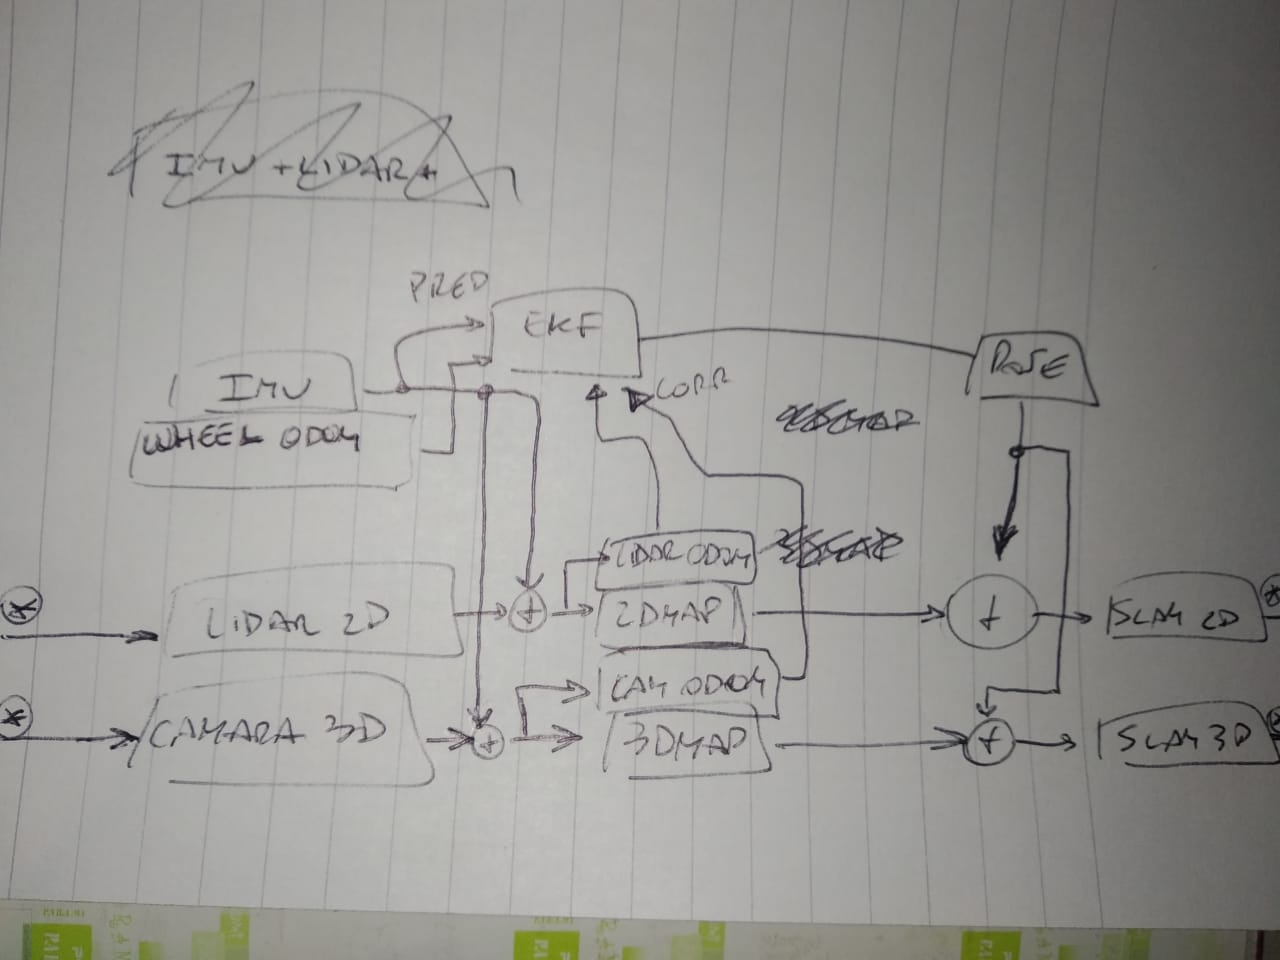
\includegraphics[width=\textwidth]{Img/SLAMAlgorithmBlockDiagram.jpeg}
    \caption{Diagrama en bloques del algoritmo SLAM propuesto}
    \label{fig:slamalgorithmblockdiagram}
\end{figure}

A continuación se presentarán los distintos algoritmos utilizados, al principio como cada uno por separado, para luego juntarlos en el EKF final.

\subsubsection{SLAM 2D}

\subsubsection{SLAM 3D}
\fi
Una vez con las nubes de puntos de profundidad provenientes de la cámara, el próximo paso refiere a la generación del mapa y la localización del robot en el entorno, utilizando el denominado \textit{registration pipeline} (presentado en la Sección \ref{sec:marcoteorico}). A continuación, se desarrollan los pasos realizados a estas nubes de puntos, los cuales pueden verse en la Figura \ref{fig:3dalgorithmblockdiagram}.

\begin{figure}
    \centering
    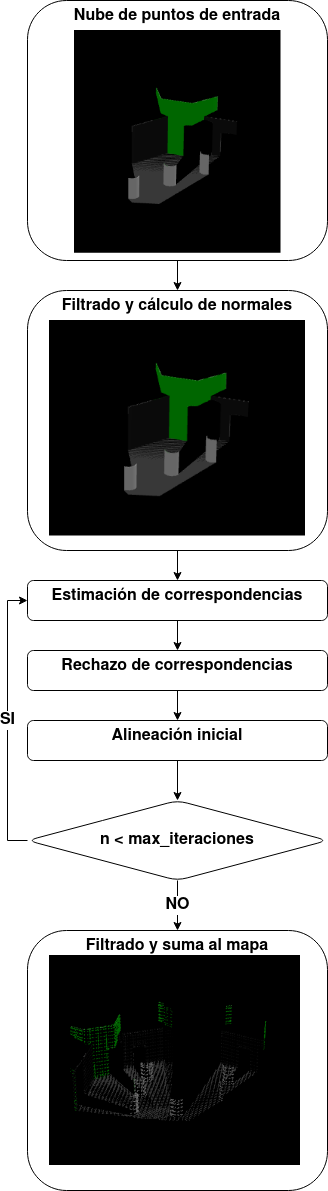
\includegraphics[scale=0.45]{Img/3DAlgorithmBlockDiagram.png}
    \caption{Diagrama en bloques del pipeline realizado para el registro de nube de puntos tridimensionales y su posterior actualización del mapa 3D}
    \label{fig:3dalgorithmblockdiagram}
\end{figure}

\subsubsection{Etapa de selección de datos}
Debido a que se utiliza una resolución de 640x480, hay una gran cantidad de puntos, haciendo que el costo computacional sea muy alto por cada corrida del algoritmo. Para ello, lo primero que se hace es un filtrado de dichos datos. Tal como se menciona en \cite{holz2015}, es importante conservar los bordes, por lo que el filtro bilateral es una buena opción. En PCL es implementado mediante \lstinline{pcl::FastBilateralFilter}.

Como vimos en la Sección \ref{sec:marcoteorico}, las normales de los puntos ayudan no solo en la etapa de rechazo de correspondencias, sino también puede ser útil en la etapa de filtrado, como es el caso de \textit{normal space sampling}. Debido a que los datos originales son del tipo \lstinline{pcl::PointXYZRGB}, es necesario calcular dichas normales. Un método rápido para hacer esto es mediante el uso de imágenes integrales \cite{holzer2012}. La ventaja de este método es que solo requiere una etapa de preprocesamiento lineal al tiempo que permite calcular los vectores medios y las normas dentro de un área rectangular de la imagen en tiempo constante. Por lo tanto, en primera instancia mediante la implementación de PCL \lstinline{pcl::IntegralImageNormalEstimation} se calculan las normales, para luego realizar el \textit{normal space sampling}.

Como el algoritmo de \textit{normal space sampling} requiere de una nube de puntos ordenada, luego de este proceso se procede a la remoción de los datos inválidos de las nubes de puntos, mediante la implementación de PCL \lstinline{pcl::removeNaNFromPointCloud}.

\subsubsection{Estimación de correspondencias}
Una vez obtenidos los puntos filtrados y con sus respectivas normales (dando lugar entonces a puntos del tipo \lstinline{pcl::PointXYZRGBNormal}), se procede al cálculo de las correspondencias entre las nubes de puntos.

\subsubsection{Rechazo de correspondencias}
Como se tienen tanto los datos de la posición como de la normal de cada punto, se emplean dos filtros de correspondencias
\begin{itemize}
    \item uno para filtrar la distancia mediante el uso de la mediana, dando lugar al \lstinline{pcl::registration::CorrespondenceRejectorMedianDistance}, y
    \item  un segundo filtro en base a las superficies normales, esto es, \lstinline{pcl::registration::CorrespondenceRejectorSurfaceNormal}, asignando un peso a las correspondencias en base al error que presentan las cámaras RGB-D \cite{nguyen2012}, el cual puede generalizarse al modelo presente en la Ecuación \ref{eq:weightcorrespondences}, considerando dos puntos $\bm{p}$ y $\bm{q}$
    \begin{align}
        w(\bm{p},\bm{q}) &= max(\sigma_z({\bm{p}_z}), \sigma_z(\bm{q}_z))
        \label{eq:weightcorrespondences} \\
        \text{con }\sigma_z(z) &= 0.0012+0.0019\cdot (z-0.4)^2
    \end{align}
\end{itemize}

En concreto, primero se realiza el filtro de mediana, y luego el filtro en base a la información de las normales.

\subsubsection{Alineación}
Finalmente, con las correspondencias restantes se procede al cálculo de la transformación que responde a las dos nubes de puntos. Para ello, se utiliza el principio de punto a plano, debido a su rápida convergencia y buena precisión comparado con el método de punto a punto. Por ello, utilizando la función de PCL \lstinline{pcl::registration::TransformationEstimationPointToPlaneWeighted} se llega a la transformación que describe en una primera instancia el movimiento realizado por el robot.

\subsubsection{Refinamiento y actualización}
Debido a los posibles mínimos locales encontrados en lugar del mínimo global, para poder encontrar la transformación adecuada, se itera en los pasos de estimación de correspondencias, el rechazo de las mismas y el cálculo de la transformada, realizando la transformación de la nube de puntos fuente (filtrada y con sus respectivas normales) en base al resultado anterior, para luego calcular dichos valores nuevamente.

Finalmente, con la tranformación calculada se aplica la misma a la nube de puntos fuente para, luego de un nuevo filtrado para reducir su tamaño, agregarla al mapa generado en base a las nubes de puntos previas. En PCL, haciendo simplemente una suma de dicha nube de puntos transformada con el mapa se consigue el objetivo.

\subsection{Resultados}
Debido a los problemas mencionados de la cámara Minoru para generar los mapas, sumado a que no se dispone del dato real de la trayectoria del robot para poder contrastarla con el algoritmo desarrollado, se cambió el enfoque del trabajo y se optó por obtener los datos en base a un entorno de simulación que, como se mencionó anteriormente, fue Gazebo el elegido. 

Dentro de los modelos que se encuentran disponibles, se tomó el modelo del robot terrestre  \textit{Rosbot 3.0}\footnote{https://github.com/husarion/rosbot\_description} para realizar las simulaciones, el cual cuenta con una Microsoft Kinect, además de contar con un LIDAR 2D, IMU y encoders. A su vez, el mismo fabricante proporciona mapas simulados para la realización de pruebas, y con el agregado de los mapas presentes en el robot \textit{Turtlebot3}\footnote{https://github.com/ROBOTIS-GIT/turtlebot3} se consiguen una suficiente cantidad de entornos para ensayar el algoritmo descripto. A continuación, se detallan los resultados en base a uno de los mapas y el \textit{Rosbot 3.0}.

Para el caso, se evaluó el mapa \textit{turtlebot3 world}, que se observa en la Figura \ref{fig:turtlebotworldoriginalmap}, además de observarse también el modelo simulado del Rosbot 3.0. A partir de dicha simulación, se movió al robot sin un patrón específico, tratando de que pueda mapearse todo el lugar, guardando los tópicos de interés en un contenedor de ROS (\textit{rosbag}) para luego poder procesar y evaluar la misma información con el fin de poder ajustar el algoritmo. En base a esto, se fue construyendo el mapa con cada una de las nubes de puntos entrantes, comparado a cada una con la nube de puntos anterior y sumando entonces la nueva nube transformada al mapa generado, mediante el \textit{registration pipeline} descrito anteriormente. En base a esto, se consiguieron los resultados que se observan en la Figura \ref{fig:turtlebotworldestimatedmap}, donde la traza roja representa a la trayectoria real del robot (dato proporcionado por la simulación), mientras que la trayectoria azul se trata de la trayectoria estimada por el algoritmo realizado.
\begin{figure}[!ht]
    \centering
    {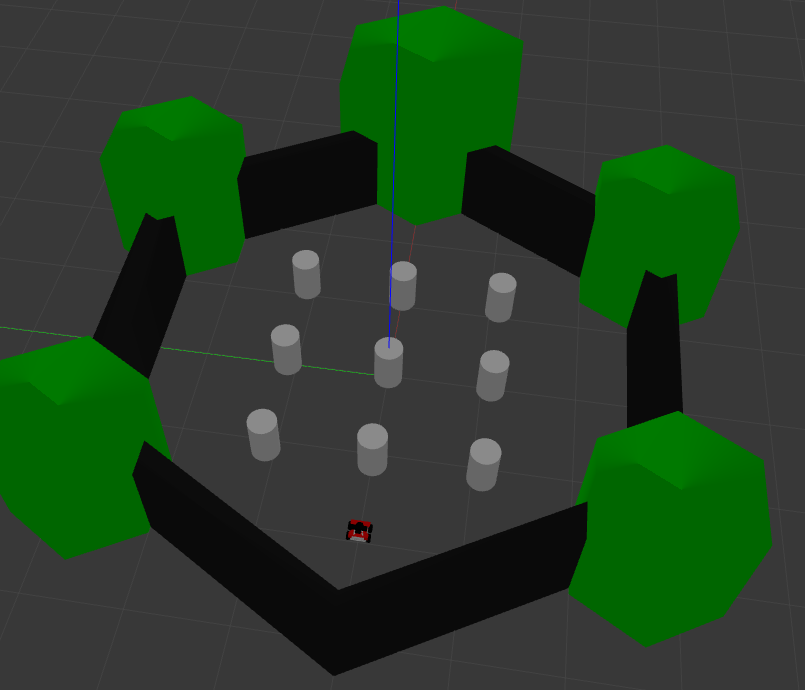
\includegraphics[width=\linewidth]{Img/TurtleBotWorldMap3D.png}}
    \caption{Entorno simulado \textit{turtlebot3 world}}
    \label{fig:turtlebotworldoriginalmap}
\end{figure}
\begin{figure}[!ht]
    \centering
    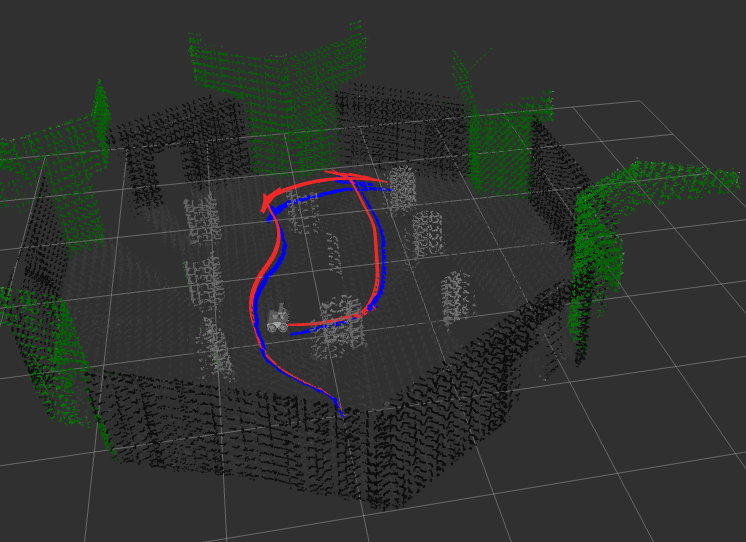
\includegraphics[width=\linewidth]{Img/TurtleBotWorldMap3DEstimated.png}%
    \caption{Mapa reconstruido en base a la cámara RGB-D del entorno simulado, junto a la trayectoria real y estimada por el algoritmo}
    \label{fig:turtlebotworldestimatedmap}
\end{figure}
Como el tiempo de procesamiento en una computadora de 4 núcleos (2.0 GHz) ronda el segundo, se redujo la tasa de ejecución del contenedor de ROS para poder procesar todas las nubes de puntos, ya que se consiguen datos cada medio segundo. 


Como se pretende realizar luego una fusión sensorial, combinando un LIDAR 2D y una IMU, una opción para que pueda llevarse al tiempo real es procesando cada cierto tiempo las nubes, ignorando entonces parte de ellas. Como el LIDAR 2D da información respecto a la pose del vehículo, se conseguirían entonces resultados aproximados, ya que para cada paso del algoritmo se partiría de la última transformación estimada, ya sea de la cámara, del LIDAR o de un algoritmo externo, como puede ser el filtro de Kalman.